\section{Plano lateral}
\label{sec:plano_lateral}

No plano do braço, como é possível observar na Figura~\ref{fig:lateral}, a posição da garra exprime-se em dois eixos: $d$, a distância em frente, e $h$, a altura acima da base. Neste plano, J2, J3 e J4 têm eixos de rotação paralelos entre si, perpendiculares ao plano, e por isso o braço comporta-se como o braço planar estudado na aula.

\begin{figure}[h]
  \centering
  \resizebox{0.6\textwidth}{!}{%Vista lateral do robô
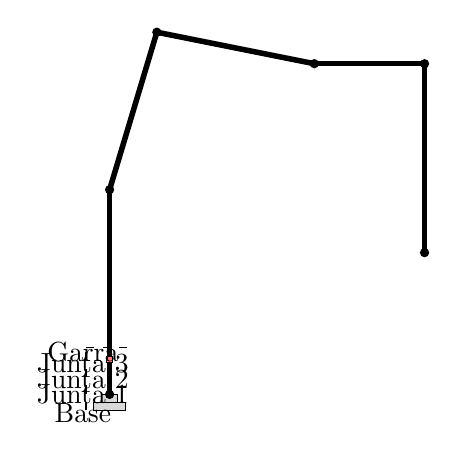
\begin{tikzpicture}[scale=0.2,
                    % Estilos
                    link/.style={line width=2pt, line cap=round},
                    junta/.style={circle, draw, fill=blue!50, line width=1pt, inner sep=2pt}]

  % Coordenadas das juntas
    \coordinate (J1) at (1,1);
    \coordinate (J2) at (1,14);
    \coordinate (J3) at (4,24);
    \coordinate (J4) at (14,22);
    \coordinate (J5) at (21,22);
    \coordinate (J6) at (21,10);

  % Base
    \draw[fill=gray!30] (0,0) rectangle (2,0.5);
    \draw[fill=gray!30] (0.5,0.5) rectangle (1.5,1);
  
  % Juntas
    \draw[junta] (J1) circle (0.2);
    \draw[junta] (J2) circle (0.2);
    \draw[junta] (J3) circle (0.2);
    \draw[junta] (J4) circle (0.2);
    \draw[junta] (J5) circle (0.2);
    \draw[junta] (J6) circle (0.2);
  
  % Braços
    \draw[link] (J1) -- (J2);
    \draw[link] (J2) -- (J3);
    \draw[link] (J3) -- (J4);
    \draw[link] (J4) -- (J5);
    \draw[link] (J5) -- (J6);
  
  % Garra
  \draw[fill=red!50] (0.8,3) rectangle (1.2,3.4);
  
  % Eixos
  \draw[dashed] (-0.5,0) -- (-0.5,4);
  \draw[dashed] (-0.5,4) -- (2.5,4);
  
  % Labels
  \node at (-0.7,-0.2) {Base};
  \node at (-0.7,1) {Junta 1};
  \node at (-0.7,2) {Junta 2};
  \node at (-0.7,3) {Junta 3};
  \node at (-0.7,3.7) {Garra};
\end{tikzpicture}}
  \caption{Vista lateral do braço no seu plano vertical.}
  \label{fig:lateral}
\end{figure}

\subsection{Ângulos absolutos}

Os ângulos das juntas $q_i$ são \underline{relativos}: cada um mede a rotação de um elo em relação ao elo anterior, com o sentido anti-horário positivo. Para somar as projeções de cada elo é mais simples usar ângulos \underline{absolutos}, medidos a partir da horizontal. Como no exemplo do braço de 3 DOF da aula, o ângulo absoluto de cada elo é a soma dos ângulos das juntas anteriores.

Na pose zero (todas as juntas a $0^\circ$) o braço está na vertical, por isso o primeiro elo faz $90^\circ$ com a horizontal quando $q_2 = 0$. A garra é perpendicular ao elo $L_4$. Daqui resultam:
\begin{equation}
    \theta_A = q_2 + \frac{\pi}{2}, \qquad
    \theta_B = \theta_A + q_3, \qquad
    \theta_C = \theta_B + q_4, \qquad
    \alpha = \theta_C - \frac{\pi}{2}
    \label{eq:angulos}
\end{equation}
onde $\theta_A$, $\theta_B$ e $\theta_C$ são os ângulos de $L_2$, $L_3$ e $L_4$ com a horizontal, e $\alpha$ é o ângulo da garra. Com $\alpha = -90^\circ$ a garra aponta na vertical para baixo.

\subsection{Posição de cada junta}

Partindo da base e somando, elo a elo, a projeção horizontal ($L\cos\theta$) e vertical ($L\sin\theta$) de cada elo, obtém-se a posição de cada junta no plano do braço:
\begin{align}
    \text{J2 (ombro):}   \quad & (d_2,\, h_2) = (0,\; L_1) \label{eq:j2}\\
    \text{J3 (cotovelo):} \quad & (d_3,\, h_3) = (d_2 + L_2\cos\theta_A,\; h_2 + L_2\sin\theta_A) \label{eq:j3}\\
    \text{J4 (pulso):}   \quad & (d_4,\, h_4) = (d_3 + L_3\cos\theta_B,\; h_3 + L_3\sin\theta_B) \label{eq:j4}\\
    \text{J5:}           \quad & (d_5,\, h_5) = (d_4 + L_4\cos\theta_C,\; h_4 + L_4\sin\theta_C) \label{eq:j5}
\end{align}

As Equações~\eqref{eq:j3} e~\eqref{eq:j4} são exatamente o braço planar de 2 DOF da aula, com $L_A = L_2$, $L_B = L_3$, $\theta_1 = \theta_A$ e $\theta_2 = q_3$:
\begin{equation}
    x_2 = L_A\cos\theta_1 + L_B\cos(\theta_1 + \theta_2), \qquad
    y_2 = L_A\sin\theta_1 + L_B\sin(\theta_1 + \theta_2)
    \label{eq:2dof}
\end{equation}
com a origem deslocada para o ombro, à altura $L_1$.

\subsection{Posição do centro de preensão}

O centro de preensão está a uma distância $D = L_6 + L_7$ de J5, ao longo da garra, ou seja, na direção $\alpha$. Somando esta última parcela às anteriores, a posição da garra no plano do braço é:
\begin{align}
    d &= L_2\cos\theta_A + L_3\cos\theta_B + L_4\cos\theta_C + D\cos\alpha \label{eq:d}\\
    h &= L_1 + L_2\sin\theta_A + L_3\sin\theta_B + L_4\sin\theta_C + D\sin\alpha \label{eq:h}
\end{align}

Estas equações têm a mesma forma que o braço de 3 DOF da aula ($x_e = L_A\cos\theta_1 + L_B\cos(\theta_1+\theta_2) + L_C\cos(\theta_1+\theta_2+\theta_3)$), com duas diferenças próprias do myCobot: a altura $L_1$ do ombro e o último elo em L, formado por $L_4$ e pela garra $D$, que fazem $90^\circ$ entre si.

\begin{figure}[H]
  \centering
  \resizebox{0.75\textwidth}{!}{\begin{tikzpicture}[scale=0.3, >=stealth,
    elo/.style={line width=2.2pt, line cap=round},
    junta/.style={circle, draw, fill=white, line width=1pt, inner sep=2pt},
    guia/.style={gray!60, thin, densely dotted},
    seg/.style={line width=2.4pt},
    every node/.style={font=\footnotesize}]
  \colorlet{cL1}{gray!70!black}
  \colorlet{cL2}{blue!70!black}
  \colorlet{cL3}{orange!85!black}
  \colorlet{cL4}{green!50!black}
  \colorlet{cD}{violet!80!black}

  % Coordenadas
  \coordinate (B)  at (0,0);
  \coordinate (J2) at (0,13.2);
  \coordinate (J3) at (4.7,23.2);
  \coordinate (J4) at (14.1,21.5);
  \coordinate (J5) at (21.0,24.0);
  \coordinate (G)  at (26.2,9.8);

  % Eixos
  \draw[->, thin] (-2,0) -- (36,0) node[below left] {$d$};
  \draw[->, thin] (B) -- (0,28) node[left] {$h$};
  \fill[gray!25] (-2.5,-0.8) rectangle (2.5,0);

  % Guias
  \foreach \P in {J3,J4,J5,G} \draw[guia] (\P) -- (\P |- 0,-2.2);
  \draw[guia] (J2) -- (29,13.2);
  \draw[guia] (J3) -- (30,23.2);
  \draw[guia] (J4) -- (31,21.5);
  \draw[guia] (J5) -- (32,24.0);
  \draw[guia] (G)  -- (33,9.8);

  % Braços
  \draw[elo, cL1] (B)  -- (J2);
  \draw[elo, cL2] (J2) -- node[left]  {$L_2$} (J3);
  \draw[elo, cL3] (J3) -- node[pos=0.55, above] {$L_3$} (J4);
  \draw[elo, cL4] (J4) -- node[above left] {$L_4$} (J5);
  \draw[elo, cD]  (J5) -- node[right] {$D$} (G);
  \foreach \P in {J2,J3,J4,J5} \node[junta] at (\P) {};
  \fill (G) circle (6pt);
  \node[left=4pt]  at (J2) {J2};
  \node[above=3pt] at (J3) {J3};
  \node[below=4pt] at (J4) {J4};
  \node[above=3pt] at (J5) {J5};
  \node[below left=2pt] at (G) {garra};

  % Ângulos
  \draw[guia] (J2) -- ++(3.5,0);  \draw[->, thin, cL2] ($(J2)+(2.5,0)$) arc[start angle=0, end angle=65, radius=2.5] node[pos=0.4, right] {$\theta_A$};
  \draw[guia] (J3) -- ++(3.5,0);  \draw[->, thin, cL3] ($(J3)+(2.8,0)$) arc[start angle=0, end angle=-10, radius=2.8] node[pos=1, below right=-1pt] {$\theta_B$};
  \draw[guia] (J4) -- ++(3.5,0);  \draw[->, thin, cL4] ($(J4)+(2.8,0)$) arc[start angle=0, end angle=20, radius=2.8] node[pos=0.6, right] {$\theta_C$};
  \draw[guia] (J5) -- ++(3.5,0);  \draw[->, thin, cD]  ($(J5)+(2.5,0)$) arc[start angle=0, end angle=-70, radius=2.5] node[pos=0.6, right] {$\alpha$};

  % Soma de d
  \draw[seg, cL2] (0,-2.2)    -- (4.7,-2.2);
  \draw[seg, cL3] (4.7,-2.2)  -- (14.1,-2.2);
  \draw[seg, cL4] (14.1,-2.2) -- (21.0,-2.2);
  \draw[seg, cD]  (21.0,-2.2) -- (26.2,-2.2);
  \node[cL2, below=3pt] at (2.35,-2.2)  {$L_2\cos\theta_A$};
  \node[cL3, above=3pt] at (9.4,-2.2)   {$L_3\cos\theta_B$};
  \node[cL4, below=3pt] at (17.55,-2.2) {$L_4\cos\theta_C$};
  \node[cD,  above=3pt] at (23.6,-2.2)  {$D\cos\alpha$};
  \draw[|<->|, thin] (0,-5.2) -- node[fill=white, inner sep=1pt] {$d$} (26.2,-5.2);

  % Soma de h
  \draw[seg, cL1, ->] (29,0)    -- (29,13.2);
  \draw[seg, cL2, ->] (30,13.2) -- (30,23.2);
  \draw[seg, cL3, ->] (31,23.2) -- (31,21.5);
  \draw[seg, cL4, ->] (32,21.5) -- (32,24.0);
  \draw[seg, cD,  ->] (33,24.0) -- (33,9.8);
  \draw[guia] (29,13.2) -- (30,13.2) (30,23.2) -- (31,23.2) (31,21.5) -- (32,21.5) (32,24.0) -- (33,24.0);
  \node[cL1, left=1pt]  at (29,6.6)   {$L_1$};
  \node[cL2, right=1pt] at (30,17.5)  {$L_2\sin\theta_A$};
  \node[cL3, right=1pt] at (33.2,22.4) {$L_3\sin\theta_B < 0$};
  \node[cL4, right=1pt] at (32,25.6)  {$L_4\sin\theta_C$};
  \node[cD,  right=1pt] at (33,15.0)  {$D\sin\alpha < 0$};
  \draw[|<->|, thin] (36,0) -- node[fill=white, inner sep=1pt] {$h$} (36,9.8);
  \draw[guia] (33,9.8) -- (36,9.8);
  
\end{tikzpicture}}
  \caption{Somas das projeções dos elos do braço.}
  \label{fig:soma_projecoes}
\end{figure}

\subsection{Juntas 5 e 6}

A junta 5 roda a garra em torno do eixo de $L_4$, tirando-a do plano do braço. Para $q_5 \neq 0$, só a componente $D\cos q_5$ fica no plano e a componente $D\sin q_5$ passa a ser um desvio lateral; as Equações~\eqref{eq:d} e~\eqref{eq:h} ficam
\begin{equation}
    d = \dots + D\cos q_5\cos\alpha, \qquad
    h = \dots + D\cos q_5\sin\alpha, \qquad
    l = L_5 - D\sin q_5
    \label{eq:q5}
\end{equation}
onde $l$ é o desvio lateral total do plano do braço. Como no projeto $q_5 = 0$, tem-se $l = L_5$. A junta 6 roda a garra em torno do seu próprio eixo e não entra nas equações da posição.

\clearpage